\chapter{Análise Bibliográfica sobre reconhecimento biométrico, por João Pedro Felix}

\section{Planejamento do estudo}
Do controle de acesso a um dispositivo celular até a autenticação de um eleitor para o uso da urna eletrônica, a biometria tem se mostrado uma das maneiras mais eficazes de garantir que alguém é de fato quem afirma ser.

Reconhecimento de digital, iris, palmar e facial são apenas algumas das maneiras mais comuns de se realizar essa identificação, que parte do princípio que, na prática, essas características podem ser consideradas únicas para cada pessoa.

Isso tudo me leva a questionar, por exemplo, os seguintes fatores:

\begin{enumerate}
    \item Quais são os conceitos mais relevantes relacionados com identificação biométrica?
    \item Quais são os métodos mais relevantes de reconhecimento biométrico?
    \item Quem são os autores mais relevantes e com quais tópicos mais específicos eles trabalham?
\end{enumerate}

\subsection{O que já existe de pesquisa bibliométrica sobre biometria?}

Um estudo bibliométrico sobre identificação biométrica a partir do movimento dos olhos foi proposto por \citet{brasil_eye_2020}, contudo, o objetivo lá apresentado é diferente daqui, uma vez que minha intenção é ter uma visão mais geral no assunto, justamente por ainda ter pouco conhecimento na área.

\subsection{Ferramentas Utilizadas}

A realização da pesquisa bibliométrica será realizada a partir da ferramenta RStudio, juntamente do pacote \textit{Bibliometrix} e do aplicativo \textit{Biblioshiny}. Os artigos que serão usados foram extraídos da base de dados \textit{Web of Science}.

\section{Coleta de Dados}

A coleta de dados foi realizada utilizando a base de dados Web of Science no dia 03/02/2022, acessada por meio do Portal de Periódicos da CAPES.

A busca foi feita utilizando as coleções Science Citation Index Expanded (SCI-Expanded)--1945-presente, Conference Proceedings Citation index - Science (CPCI-S)--1990-presente e Emergin Sources Citation Index (ESCI)--2017-presente.

\subsection{Busca e refinamento}
Inicialmente a busca realizada foi a apresentada em \ref{BIPA@DYosplayQueryBiometrics1}, que procurou por artigos que contivessem o seguinte tópico:


\lstinputlisting[numbers=left,basicstyle=\normalsize\ttfamily,caption={Pesquisa sobre biometria},label=BIPA@DYosplayQueryBiometrics1]
{experiments/DYosplay/PesquisaBibliometrica/Pesquisas/pesquisa1.txt}


A ideia inicial era encontrar artigos que tratassem de biometria e processamento de imagens, a intenção com isso era evitar em especial artigos mais focados na área de biologia por exemplo, ao priorizar os que tivessem relação direta com processamento de imagens.

Contudo, foram obtidos apenas cerca de 2000 resultados. Assim, uma nova busca foi realizada, como mostrado abaixo (em \ref{BIPA@DYosplayQueryBiometrics2}), que resultou em 5252 itens encontrados.

\lstinputlisting[numbers=left,basicstyle=\normalsize\ttfamily,caption={Pesquisa refinada sobre biometria},label=BIPA@DYosplayQueryBiometrics2]
{experiments/DYosplay/PesquisaBibliometrica/Pesquisas/pesquisa2.txt}

A melhora aconteceu ao incluir na busca os termos \textit{recognition}, que significa "reconhecimento", e \textit{verification}, que significa "verificação", como alternativa a \textit{processing} que significa "processamento", mas sem abrir mão de \textit{image}, que quer dizer "imagem". 

A ideia surgiu ao observar que alguns dos resultados obtidos a partir da primeira busca possuíam essas duas palavras em seus títulos e que por vezes eram utilizadas no mesmo contexto que "processamento".

Os registros foram exportados via arquivo de texto sem formatação com todos os 29 campos disponíveis. É importante ressaltar a presença do campo "referências citadas", que permite a análise das citações.

Por limitações da plataforma, os registros foram exportados em cinco arquivos com mil registros cada e um arquivo com 252 registros. Em seguida, todos esses arquivos foram concatenados na ordem que foram exportados, resultando em um novo arquivo contendo os 5252 registros.

O arquivo final pode ser consultado no GitHUB do projeto a partir desse \href{https://github.com/jhcf/Comput-Experim-20212/tree/main/experiments/DYosplay/PesquisaBibliometrica/Registros}{link} 

\section{Análise de Dados}

\subsection{Filtragem de Registros}

Conforme sugerido em sala, os registros foram filtrados de modo a selecionar artigos propriamente ditos, excluindo assim, por exemplo, capítulos de livro e fontes em geral em acesso antecipado. Dessa forma, restaram 2014 registros, com publicações variando entre 1993 e 2022 e um total de 1838 citações, que de agora em diante serão chamados de BiometricImageProcessing/Article ou BIPA@DYosplay.

A figura \ref{fig:CoOcurrence1993-2022:BIPA@DYosplay} mostra as principais palavras chaves presentes no conjunto de dados após a filtragem. Nela, percebemos a presença de termos como reconhecimento facial, impressão palmar, digital e reconhecimento de íris, além de técnicas de reconhecimento biométrico como autofaces, extração de características, segmentação e fusão, o que mostra que, de fato, os resultados condizem com o esperado.

\begin{figure}[H]
    \centering
    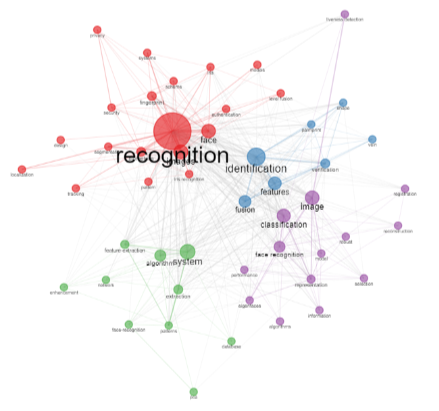
\includegraphics[width=1\textwidth]{experiments/DYosplay/PesquisaBibliometrica/Imagens/BIPA@DYosplay_CoOcurrenceNetwork1993-2022.png}
    \caption{Co-ocorrência de palavras-chaves no conjunto de dados BIBA@DYosplay no período de 1993 até 2022.}
    \label{fig:CoOcurrence1993-2022:BIPA@DYosplay}
\end{figure}


\subsection{Análise Descritiva da base de dados BIPA@DYosplay}

Abaixo se encontram as informações mais gerais da base de dados BIPA@DYosplay.

\begin{description}
    \item [``Timespan''] Após a pesquisa e filtragem os artigos resultantes foram publicados entre 1993 e 2022.
    
    \item [``Sources (Journals, Books, etc)]" No total 513 fontes de informação diferentes estão presentes na base de dados, o que dá uma média de quase 4 artigos para cada fonte de informação.
    
    \item [``Average years from publication'']  A média de tempo de publicação dos artigos é de 6,07 anos.
    
    \item [``Average citations per documents''] A média de citações por documento é de 19,17.
    
    \item [``Average citations per year per doc''] A média de citações por ano de cada artigo, a contar de sua data de publicação, é de 2,057.
    
    \item [ "References''] O conjunto de dados contém 45.581 referências citadas.
    
    \item [``Keywords Plus (ID)" ] 1.422 palavras-chaves distintas aparecem no conjunto de dados.
    
    \item [``Author's Keywords (DE)''] 5.650 palavras-chaves indicadas pelos autores estão presentes no conjunto de dados.
    
    \item [``Authors''] 5.040 nomes distintos de autores foram encontrados na base de dados.
    
    \item [``Author Appearances''] os 5.040 autores aparecem em 7.248 ocorrência pelo conjunto de  dados.
    
    \item [``Authors of single-authored documents''] Dos 5.040 autores encontrados, 79 assinam a autoria do artigo individualmente.
    
    \item [``Authors of multi-authored documents''] Dos 5.040 autores encontrados, 4961 editaram artigos em conjunto.
    
    \item [``Single-authored documents''] 88 artigos foram feitos por um único autor. Os demais foram feitos por mais de um autor.
    
    \item [``Documents per Author''] Cada um dos 5.040 nomes distintos de autores encontrados publicou em média 0.4 artigos.
    
    \item [``Authors per Document''] A média de autores por documento no conjunto de dados é de 2,5
    
    \item [``Co-Authors per Documents''] A média de co-autores por documento é de 3,6.
    
    \item [``Collaboration Index''] Os 5.040 nomes de autores encontrados colaboraram em média 2,58 vezes para editar os  1.926 artigos elaborados em co-autoria.
    
\end{description}

\subsection{Evolução da Produção Científica}
\label{DYosplay_prodcient}
A figura \ref{fig:evol:anual:BIPA@DYosplay} mostra a evolução da produção cientifica com base nos artigos sobre biometria presentes no conjunto de dados BIPA@DYosplay.

\begin{figure}[H]
    \centering
    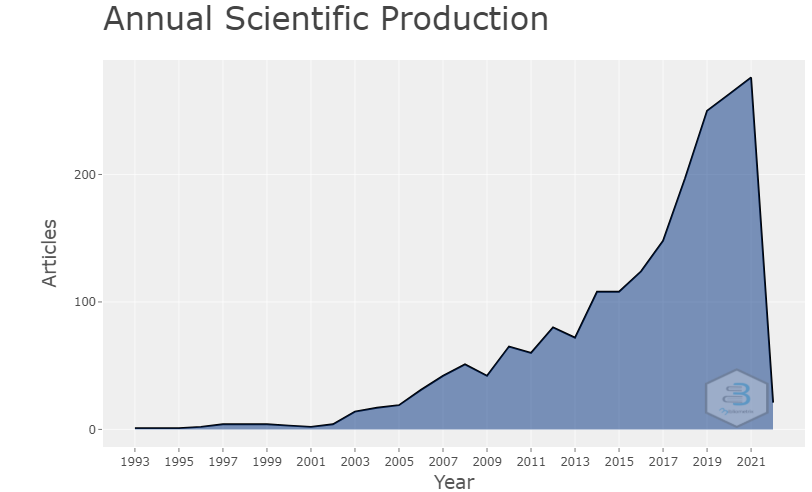
\includegraphics[width=1\textwidth]{experiments/DYosplay/PesquisaBibliometrica/Imagens/BIPA@DYosplay_Annual Scientific Production.png}
    \caption{Evolução da produção científica no conjunto de dados BIPA@DYosplay.}
    \label{fig:evol:anual:BIPA@DYosplay}
\end{figure}

A taxa de crescimento é de 11.07\% ao ano, o que justifica o formato exponencial da curva.

Os registros começam a partir do ano de 1993 e permanecem relativamente constantes até 2002, com um suave crescimento seguido de queda entre os anos de 1997 e 1999.

É só a partir de 2002, quase 10 anos após o início das publicações presentes no conjunto de dados que o crescimento se demonstra mais significativo, aumentando consideravelmente ano após ano até 2008, que marca o início de uma queda na produção científica, ao menos no que diz respeito a esse conjunto de dados.

Entre 2008 e 2014 percebemos que o comportamento se repete: um aumento seguido de queda, novamente seguido de um aumento e assim sucessivamente.

Entre 2014 e 2015 a produção se mantém estável, até que a partir de 2015 o crescimento se acentua, chegando a explodir por volta de 2017, quando acontece um crescimento sem precedentes, que se mantém até os dias de hoje.

\subsubsection{Interpretação da Curva da Evolução da Produção Científica}

A biometria é um assunto relativamente novo e tem como principal objetivo oferecer mais segurança a processos de autenticação, mas o que a curva de produção científica pode nos dizer sobre a evolução na área?

O primeiro período interessante é o que ocorre entre 1993 e 2002, período marcado pela baixa produção e que antecede o primeiro crescimento significativo. A figura \ref{fig:CoOcurrence1993-2002:BIPA@DYosplay} mostra a co-ocorrência de palavras chaves nesse período. A partir dela podemos perceber a existência de apenas duas palavras chaves principais: \textit{eigenfaces} (autofaces), que se refere ao reconhecimento de faces e \textit{templates} (modelos), relacionados com sistemas. Isso sugere que nesse período inicial o foco se concentrava principalmente em biometria facial.

\begin{figure}[H]
    \centering
    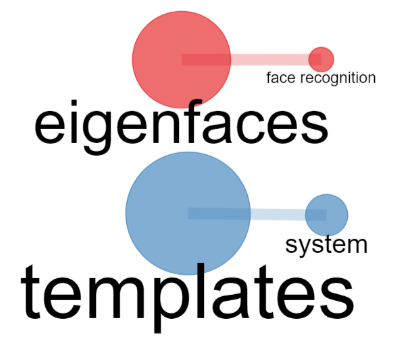
\includegraphics[width=0.5\textwidth]{experiments/DYosplay/PesquisaBibliometrica/Imagens/BIPA@DYosplay_CoOcurrenceNetwork1993-2002.png}
    \caption{Co-ocorrência de palavras chaves no período de 1993 até 2002 no conjunto de dados BIPA@DYosplay.}
    \label{fig:CoOcurrence1993-2002:BIPA@DYosplay}
\end{figure}

O segundo período interessante ocorre entre 2002 e 2015, quando observamos um maior crescimento, embora ainda com algumas baixas ocasionais.

\begin{figure}[H]
    \centering
    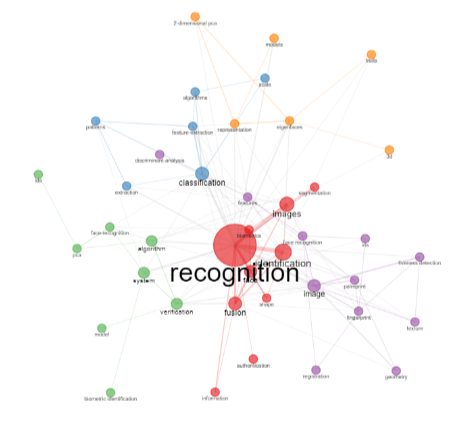
\includegraphics[width=1\textwidth]{experiments/DYosplay/PesquisaBibliometrica/Imagens/BIPA@DYosplay_CoOcurrenceNetwork2002-2015.png}
    \caption{Co-ocorrência de palavras chaves no período de 2002 até 2015 no conjunto de dados BIPA@DYosplay.}
    \label{fig:CoOcurrence2002-2015:BIPA@DYosplay}
\end{figure}

Na figura \ref{fig:CoOcurrence2002-2015:BIPA@DYosplay} observamos em destaque a palavra-chave \textit{recognition} (reconhecimento), relacionada com termos como imagens, face e autenticação, além de, é claro, biometria. Ela marca o centro do assunto, o que é totalmente compreensível. Observamos também a aparição, em vermelho, de \textit{fusion} (fusão) que, como o nome sugere, se refere a mistura de diferentes técnicas de reconhecimento biométrico para aprimorar os resultados. Outro núcleo é o presente em laranja, que possui a palavra chave \textit{eigenfaces} (autofaces), já presente nas ocorrências mostradas na figura \ref{fig:CoOcurrence1993-2002:BIPA@DYosplay}, Em verde e azul percebemos palavras-chaves como modelo, sistemas, algoritmos, extração de características e classificação, que claramente tem relação com como o processo de reconhecimento é realizado. Já em roxo percebemos os objetos sobre os quais os processos acontecerão, como reconhecimento fácil, de iris, digital e impressão palmar.

O terceiro cenário interessante de se analisar é o que compreende o período de 2017 até 2019, quando ocorre a explosão na produção.

\begin{figure}[H]
    \centering
    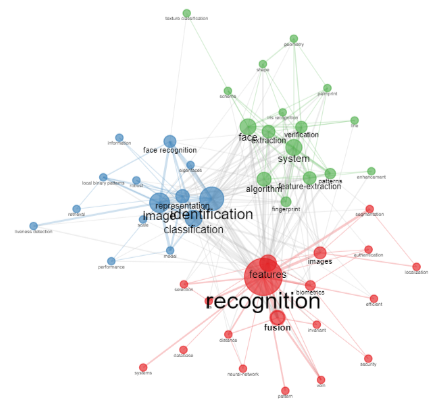
\includegraphics[width=1\textwidth]{experiments/DYosplay/PesquisaBibliometrica/Imagens/BIPA@DYosplay_CoOcurrenceNetwork2017-2019.png}
    \caption{Co-ocorrência de palavras chaves no período de 2017 até 2019 no conjunto de dados BIPA@DYosplay.}
    \label{fig:CoOcurrence2017-2019:BIPA@DYosplay}
\end{figure}

No período mostrado na figura \ref{fig:CoOcurrence2017-2019:BIPA@DYosplay} podemos observar que agora reconhecimento (\textit{recognition}) possui ligações com termos como \textit{ROI localization} (localização de regiões de interesse) e \textit{vein} (veias), o que sugere novos modelos de identificação biométrica.

\subsection{Evolução das Citações}

A figura \ref{fig:evol:anual:citacoes:BIPA@DYosplay} mostra a evolução no número de citações nos 2014 artigos presentes no conjunto de dados BIPA@DYosplay. 

Ao observar a figura percebemos que durante a maior parte do período o número de citações se mantém relativamente estável, com ocasionais picos nos anos de 1997 e 2003. Enquanto em 1997 a produção ainda era pequena, em 2003 foi quando observamos o primeiro crescimento na produção científica na área como visto na seção \ref{DYosplay_prodcient}. 

O que chama a atenção no entanto é o período inicial com alto número de citações, reflexo da baixa quantidade de artigos no momento.

\begin{figure}[H]
    \centering
    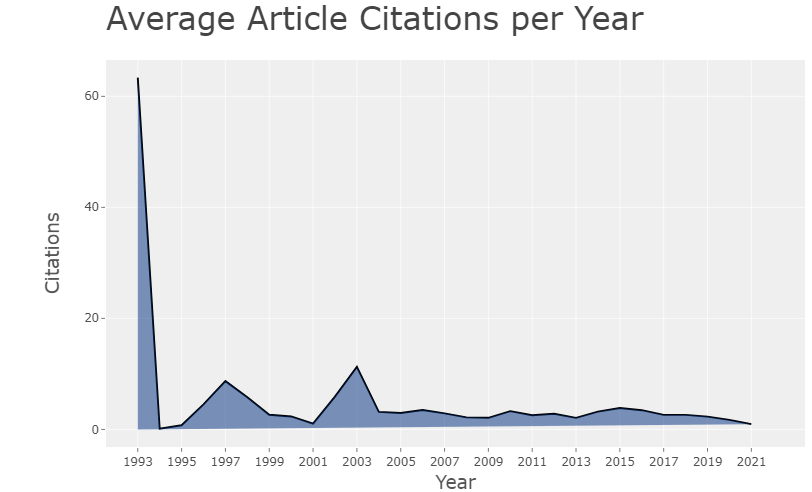
\includegraphics[width=1\textwidth]{experiments/DYosplay/PesquisaBibliometrica/Imagens/BIPA@DYosplay_Avarage Citations per Year.png}
    \caption{Evolução das citações no conjunto de dados BIPA@DYosplay.}
    \label{fig:evol:anual:citacoes:BIPA@DYosplay}
\end{figure}

\subsubsection{Interpretação da Curva de Citações por Ano}

Embora a curva de produção cientifica possua um formato exponencial, o número de citações se mantém relativamente constante ao longo de todo o período, com cada artigo no conjunto de dados sendo citado em média cerca de 3 vezes por ano.

\subsection{De onde vem essa produção científica}
\label{sec:BIPA@DYosplay_OrigemProducao}
A figura \ref{fig:MostRelevantSourcesBIPA@DYosplay} apresenta as principais fontes dos artigos presentes no conjunto de dados BIPA@DYosplay, com destaque para as revistas \textit{IEEE Transactions on Information Forensics and Security}, \textit{IEEE Acces} e \textit{Multimedia Tools and Applications}.

\begin{figure}[H]
    \centering
    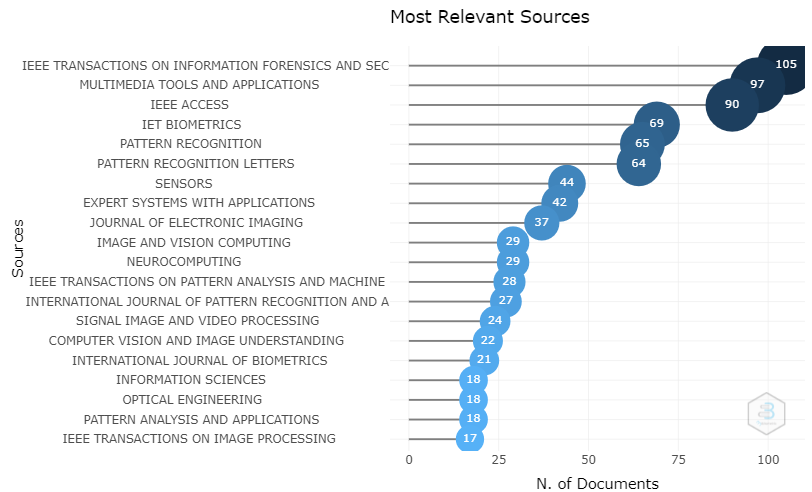
\includegraphics[width=1\textwidth]{experiments/DYosplay/PesquisaBibliometrica/Imagens/BIPA@DYosplay_MostRelevantSources.png}
    \caption{Fontes mais relevantes no conjunto de dados BIPA@DYosplay.}
    \label{fig:MostRelevantSourcesBIPA@DYosplay}
\end{figure}

A figura \ref{fig:BradfordLawBIPA@DYosplay} por sua vez mostra que o conjunto de dados BIPA@DYosplay de fato está de acordo com a lei de Bradford, que estima que os resultados de pesquisas por referências em fontes científicas tendem a diminuir exponencialmente.

Já a figura \ref{fig:MostRelevantCountriesBIPA@DYosplay} mostra os países mais citados, com destaque para a China, Estados Unidos e Inglaterra, o que faz todo sentido ao analisarmos os nomes dos autores mais relevantes na figura \ref{fig:MostRelevantAuBIPA@DYosplay} e tentarmos prever suas nacionalidades.

\begin{figure}[H]
    \centering
    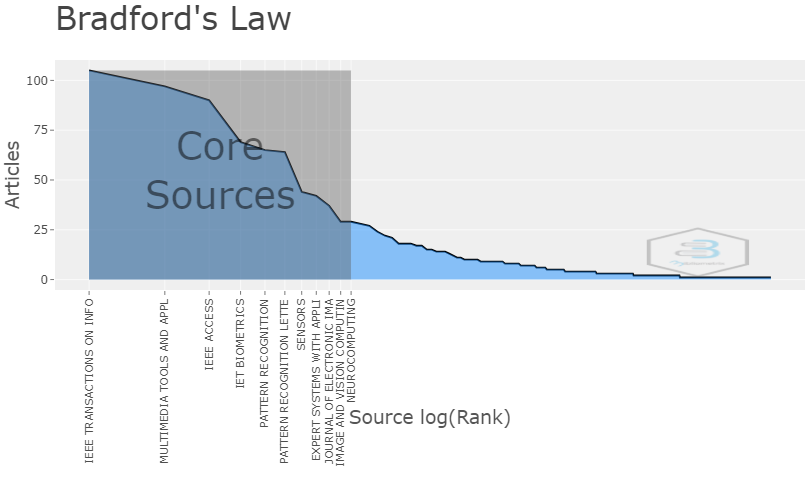
\includegraphics[width=1\textwidth]{experiments/DYosplay/PesquisaBibliometrica/Imagens/BIPA@DYosplay_BradfordLaw.png}
    \caption{Lei de Bradford no conjunto de dados BIPA@DYosplay.}
    \label{fig:BradfordLawBIPA@DYosplay}
\end{figure}

\begin{figure}[H]
    \centering
    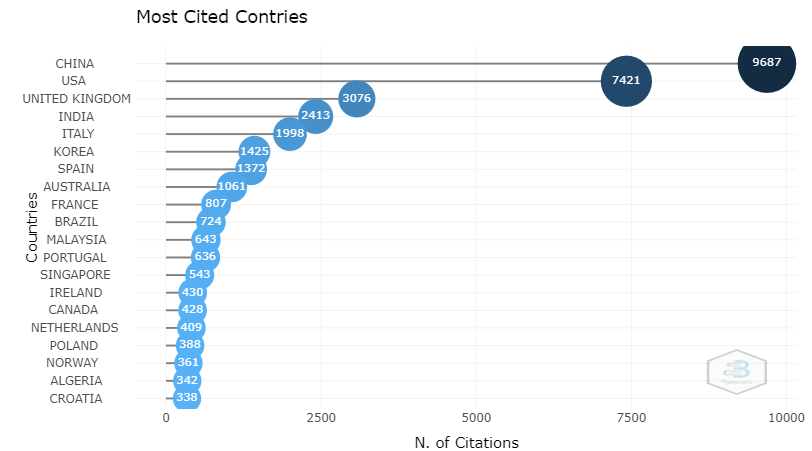
\includegraphics[width=1\textwidth]{experiments/DYosplay/PesquisaBibliometrica/Imagens/BIPA@DYosplay_MostRelevantCountries.png}
    \caption{Países mais citados no conjunto de dados BIPA@DYosplay.}
    \label{fig:MostRelevantCountriesBIPA@DYosplay}
\end{figure}

\begin{figure}[H]
    \centering
    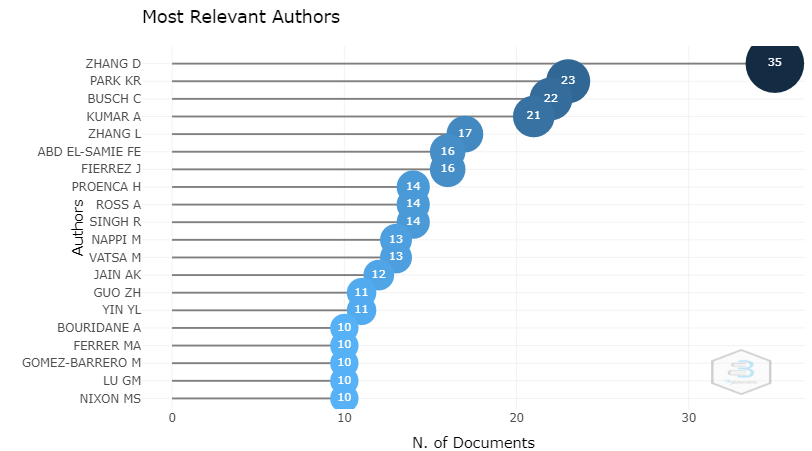
\includegraphics[width=1\textwidth]{experiments/DYosplay/PesquisaBibliometrica/Imagens/BIPA@DYosplay_MostRelevantAu.png}
    \caption{Autores mais relevantes no conjunto de dados BIPA@DYosplay.}
    \label{fig:MostRelevantAuBIPA@DYosplay}
\end{figure}

\subsection{Os artigos mais relevantes}
\label{sec:BIPA@DYosplayArtigosMaisRelevantes}

O gráfico da figura \ref{fig:GLOBALBIPA@DYOSPLAY} mostra os artigos mais citados, bem como o número de citações, do conjunto de dados BIPA@DYosplay globalmente na base de dados da \textit{Web of Science}. Isso significa que o gráfico em questão leva em conta todos os artigos presentes na \textit{Web of Science}, não se limitando aos presentes no conjunto de dados BIPA@DYosplay.

No gráfico percebemos que o artigo com maior destaque é de autoria de J. G. Daugman, seu título é: \textit{High confidence visual recognition of persons by a test of statistical independence}, que descreve um método rápido de reconhecimento biométrico a partir da íris da pessoa utilizando decisões estatísticas a partir de comparações com OU-exclusivos.

\begin{figure}[H]
    \centering
    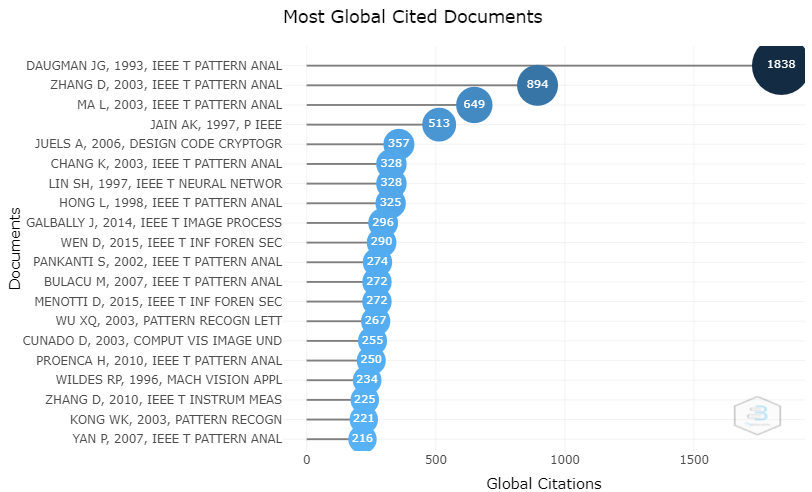
\includegraphics[width=1\textwidth]{experiments/DYosplay/PesquisaBibliometrica/Imagens/BIPA@DYosplay_GlobalArticles.png}
    \caption{Documentos no conjunto BIPA@DYosplay mais citados globalmente na \textit{Web of Science}}
    \label{fig:GLOBALBIPA@DYOSPLAY}
\end{figure}


Já a figura \ref{fig:LOCALBIPA@DYOSPLAY} apresenta os artigos mais citados, bem como o número de citações, internamente no conjunto de dados BIPA@DYosplay.

Note que o artigo mais citado é o mesmo que aparece no topo da figura \ref{fig:GLOBALBIPA@DYOSPLAY}, com praticamente o triplo das citações do segundo colocado. É interessante notar que o ano de publicação desse artigo é 1993, o que evidencia a sua importância dentro da área, assim como a relevância do autor.

\begin{figure}[H]
    \centering
    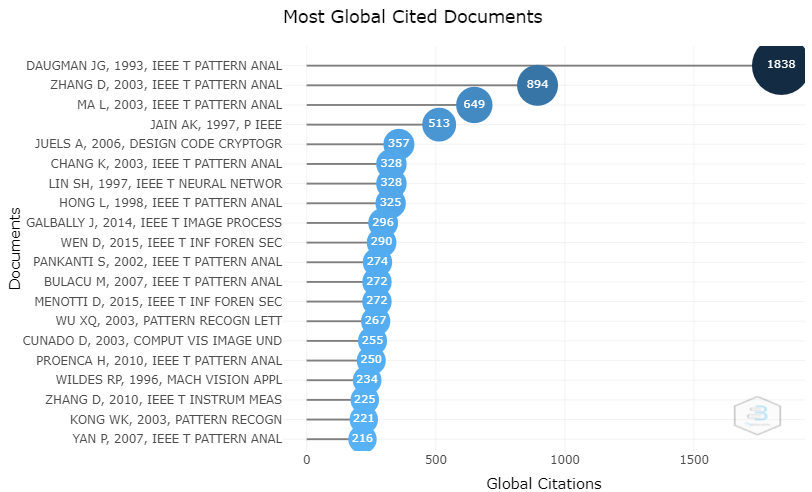
\includegraphics[width=1\textwidth]{experiments/DYosplay/PesquisaBibliometrica/Imagens/BIPA@DYosplay_GlobalArticles.png}
    \caption{Documentos no conjunto BIPA@DYosplay mais citados localmente}
    \label{fig:LOCALBIPA@DYOSPLAY}
\end{figure}


\subsection{Plotagem de Três-Campos (Diagrama de Sankey)}
\label{sec:BIPA@DYosplayPlotagemTresCampos}

A figura \ref{fig:TFP10BIPA@DYOSPLAY} apresenta a afinidade entre três conjuntos de atributos. No conjunto da esquerda se encontram as 20 citações mais frequentes (CR - \textit{Cited Record}s). No centro, encontram-se os 10 autores com maior destaque no conjunto (AU - \textit{Authors}). À direita se encontram as 20 palavras-chaves que mais aparecem (DE - \textit{Author Keywords}).

\begin{figure}[H]
    \centering
    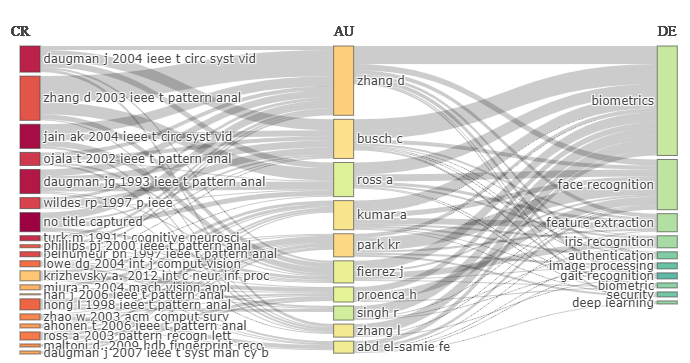
\includegraphics[width=1\textwidth]{experiments/DYosplay/PesquisaBibliometrica/Imagens/BIPA@DYosplay_Three-FieldsPlot10.png}
    \caption{Plotagem de três-campos no conjunto de dados BIPA@DYosplay}
    \label{fig:TFP10BIPA@DYOSPLAY}
\end{figure}

\subsubsection{Interpretação da Plotagem de Três-Campos}

Ao analisarmos a figura logo percebemos que "\textit{biometrics}" é a palavra-chave mais recorrente, porém se olharmos com mais atenção as demais palavras notaremos que a palavra-chave "\textit{biometric}" também aparece, o que sugere que o termo é, na realidade, ainda mais relevante. Como era de se esperar, todos os autores possuem uma conexão com o termo, diferente do último, "\textit{deep learning}", que além de aparecer pouco não está relacionado a todos os autores. Isso aconteceu devido a pesquisa ter sido objetiva, evitando, por exemplo, artigos que aparentassem ter um foco muito mais centrado em algoritmos de inteligência artificial que biometria.

Outro termo que aparece pouco é "\textit{security}", que se refere a segurança computacional e apresenta, em especial, uma ligação com autenticação. Os outros termos que aparecem eram completamente esperados dado o diagrama de co-ocorrência visto na figura \ref{fig:CoOcurrence1993-2022:BIPA@DYosplay}

Entre os autores percebemos que o mais relevante apresenta ligações com praticamente todos os termos e citam praticamente todos os registros no diagrama. Além disso, vale destacar que dois deles aparentam ter origem chinesa de acordo com o nome, enquanto não fica muito clara a nacionalidade dos demais apenas pelo nome. Outro fator interessante é que o registro mais citado é justamente o do autor com maior destaque, sendo que o mais recente é de 2012, sugerindo que nos últimos 10 anos não surgiu nada com muito destaque na área, ao menos pelo que consta neste conjunto de dados.

\subsection{Estrutura Intelectual}

\begin{figure}[H]
    \centering
    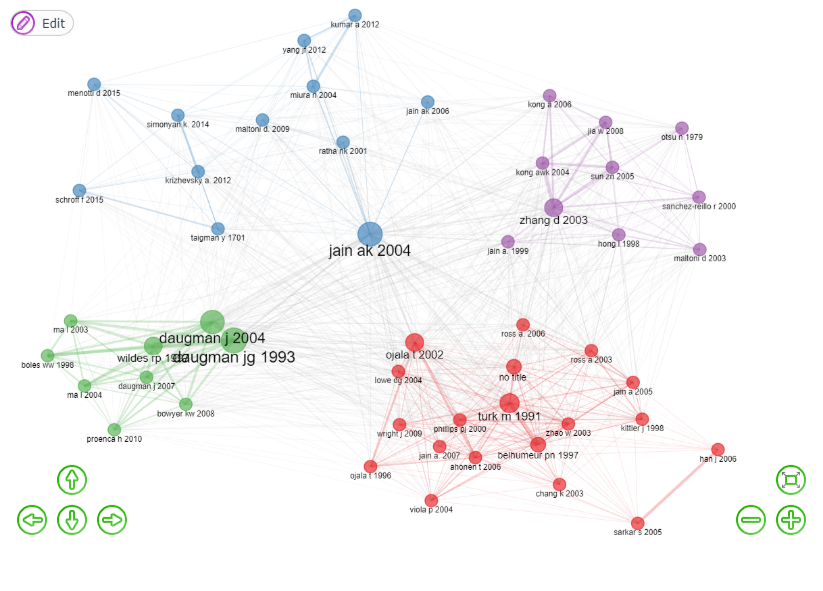
\includegraphics[width=1\textwidth]{experiments/DYosplay/PesquisaBibliometrica/Imagens/BIPA@DYosplay_CoCitation.png}
    \caption{Rede de co-citação de autores no conjunto de dados BIPA@DYosplay}
    \label{fig:CO_CITATION_BIPA@DYOSPLAY}
\end{figure}

A figura \ref{fig:CO_CITATION_BIPA@DYOSPLAY} mostra a rede co-citação de autores presentes no conjunto de dados BIPA@DYosplay. Nela, observamos quatro aglomerados principais. O aglomerado em verde tem como maior destaque o autor Daugman, o mesmo apresentado na seção \ref{sec:BIPA@DYosplayArtigosMaisRelevantes} responsável pelo artigo com maior número de citações abordado naquele momento.

O aglomerado em verde tem como maior destaque Zhang, que lidera na plotagem de três-campos apresentada na seção \ref{sec:BIPA@DYosplayPlotagemTresCampos}.

O aglomerado em azul tem como foco Jain, o que mostra que embora seja responsável por poucos artigos (apenas 12) conforme mostrado na seção \ref{sec:BIPA@DYosplay_OrigemProducao}, seu trabalho apresenta bastante relevância em campos específicos do reconhecimento biométrico.

O último aglomerado é o vermelho, onde percebemos dois autores com aparente igual relevância: Ojala e Turk. O curioso é que ambos não figuram na lista dos autores com mais publicações apresentada na seção \ref{sec:BIPA@DYosplay_OrigemProducao}, o que sugere que eles são responsáveis por artigos de grande importância na área de reconhecimento biométrico.

\section{Conclusões}
Além das conclusões apresentadas ao longo das seções, gostaria de ressaltar um pouco do que pude aprender e descobrir com a realização deste trabalho.

Primeiramente, vamos as respostas das perguntas motivadoras:
A primeira pergunta dizia respeito aos conceitos mais relevantes relacionados com identificação biométrica. A partir da análise da co-ocorrência de palavras chaves pude ver termos que não conhecia e com impacto significativo na área, como por exemplo "\textit{fusion}" e "\textit{eigenfaces}", que se referem respectivamente a fusão de diferentes técnicas de reconhecimento biométrico e conjunto de vetores próprios utilizados para o reconhecimento de rostos humanos. Além disso, pude confirmar algumas de minhas suspeitas quanto a estes conceitos, como a importância da extração de características (\textit{features}).

A segunda pergunta dizia respeito aos métodos mais relevantes de reconhecimento biométrico. A partir da análise de ocorrência de palavras chaves também podemos perceber a alta relevância de alguns métodos como  reconhecimento facial, impressão palmar, digital e reconhecimento de iris.

A terceira pergunta dizia respeito aos autores mais relevantes e as áreas que eles mais costumam atuar. Entre os autores já analisados no texto, destaco o papel de Daugman, responsável pela autoria do artigo com maior número de citações local e globalmente no conjunto de dados BIPA@DYosplay, que trata sobre reconhecimento via iris.

No que se refere aos aprendizados gerais, gostaria de ressaltar o próprio conceito de análise bibliométrica que inicialmente não tinha ficado claro. Inicialmente imaginava que o objetivo fosse simplesmente filtrar artigos de modo a agilizar o processo de encontrar algum que trate do assunto que se está procurando. Hoje no entanto, percebo que uma análise bibliométrica é uma ferramenta muito mais poderosa, sendo capaz de revelar os autores e artigos mais conceituados e dentre eles apontar os aspecto chaves que os cercam. Isso tem capacidade não apenas de direcionar a pesquisa, mas aumentar substancialmente a qualidade de um artigo produzido, uma vez que possibilita ter como referência o que há de melhor na área.
